\subsection{Body Separation of 5 mm}

The \(5~\mathrm{mm}\) separation case represents a stronger body-loading condition than the \(10~\mathrm{mm}\) case. By reducing the air gap between the dipole and the multilayer body model, the antenna fields interact more strongly with the lossy tissue layers. Therefore, a larger impedance shift, stronger efficiency degradation, and greater radiation-pattern modification are expected.

\subsubsection{Geometry and Simulation Setup}

The same tuned free-space dipole was used for the \(5~\mathrm{mm}\) body-separation case. The total dipole length was

\[
L = 122.0~\mathrm{mm},
\]

the wire radius was

\[
a = 0.905~\mathrm{mm},
\]

and the center feed gap was

\[
g = 2.0~\mathrm{mm}.
\]

The separation distance was again defined as the air gap between the lower surface of the cylindrical dipole wire and the top surface of the skin layer. Since the lower surface of the wire is located at

\[
z=-0.905~\mathrm{mm},
\]

the top of the skin layer for the \(5~\mathrm{mm}\) case was placed at

\[
z_{\mathrm{skin,top}}=-(5+0.905)
=
-5.905~\mathrm{mm}.
\]

The skin, fat, and muscle layers were stacked below this coordinate in the negative \(z\)-direction. The corresponding layer coordinates were summarized in Table~\ref{tab:body-5mm-coordinates}. The tissue material properties, finite body patch dimensions, frequency range, solver settings, and boundary conditions were kept the same as in the \(10~\mathrm{mm}\) case.

The CST time-domain solver was used over the frequency range

\[
0.7~\mathrm{GHz} \leq f \leq 1.5~\mathrm{GHz},
\]

and the far-field monitor was defined at

\[
f_0 = 1.120~\mathrm{GHz}.
\]

The CST geometry for the \(5~\mathrm{mm}\) separation case is shown in Figure~\ref{fig:body-5mm-geometry}.

\begin{figure}[htbp]
\centering
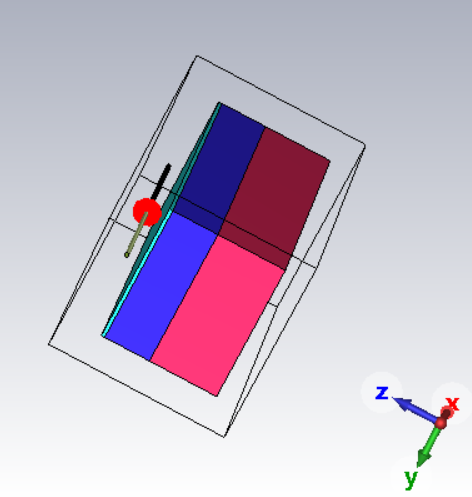
\includegraphics[width=0.82\textwidth]{figures/body_5mm/geometry_body_5mm_side_view.png}
\caption{CST side-view geometry for the \(5~\mathrm{mm}\) antenna-body separation case.}
\label{fig:body-5mm-geometry}
\end{figure}

\subsubsection{Return-Loss Result}

The CST return-loss result for the \(5~\mathrm{mm}\) body-separation case showed a stronger downward shift of the matching minimum compared with the \(10~\mathrm{mm}\) case. The minimum \(S_{11}\) occurred at

\[
f_{\min} = 0.9792~\mathrm{GHz},
\]

with

\[
S_{11,\min} = -11.9744~\mathrm{dB}.
\]

At the design target frequency,

\[
f_0 = 1.120~\mathrm{GHz},
\]

the return loss was

\[
S_{11}(1.120~\mathrm{GHz}) = -5.903831~\mathrm{dB}.
\]

\begin{table}[htbp]
\centering
\caption{Return-loss result for the \(5~\mathrm{mm}\) body-separation case.}
\label{tab:body-5mm-s11-result}
\begin{tabular}{lc}
\hline
\textbf{Quantity} & \textbf{Value} \\
\hline
Dipole length & \(122.0~\mathrm{mm}\) \\
Antenna-body separation & \(5~\mathrm{mm}\) \\
Minimum-\(S_{11}\) frequency & \(0.9792~\mathrm{GHz}\) \\
Minimum \(S_{11}\) & \(-11.9744~\mathrm{dB}\) \\
\(S_{11}\) at \(1.120~\mathrm{GHz}\) & \(-5.903831~\mathrm{dB}\) \\
\hline
\end{tabular}
\end{table}

Compared with the \(10~\mathrm{mm}\) case, the matching minimum moved from

\[
1.0312~\mathrm{GHz}
\]

to

\[
0.9792~\mathrm{GHz}.
\]

This additional downward shift confirms that reducing the antenna-body separation increases the effective dielectric loading of the dipole. At the target frequency, the return loss also degraded from

\[
-7.839072~\mathrm{dB}
\]

for the \(10~\mathrm{mm}\) case to

\[
-5.903831~\mathrm{dB}
\]

for the \(5~\mathrm{mm}\) case.


The return-loss response for the \(5~\mathrm{mm}\) body-loading case is shown in Figure~\ref{fig:body-5mm-s11}.

\begin{figure}[htbp]
\centering
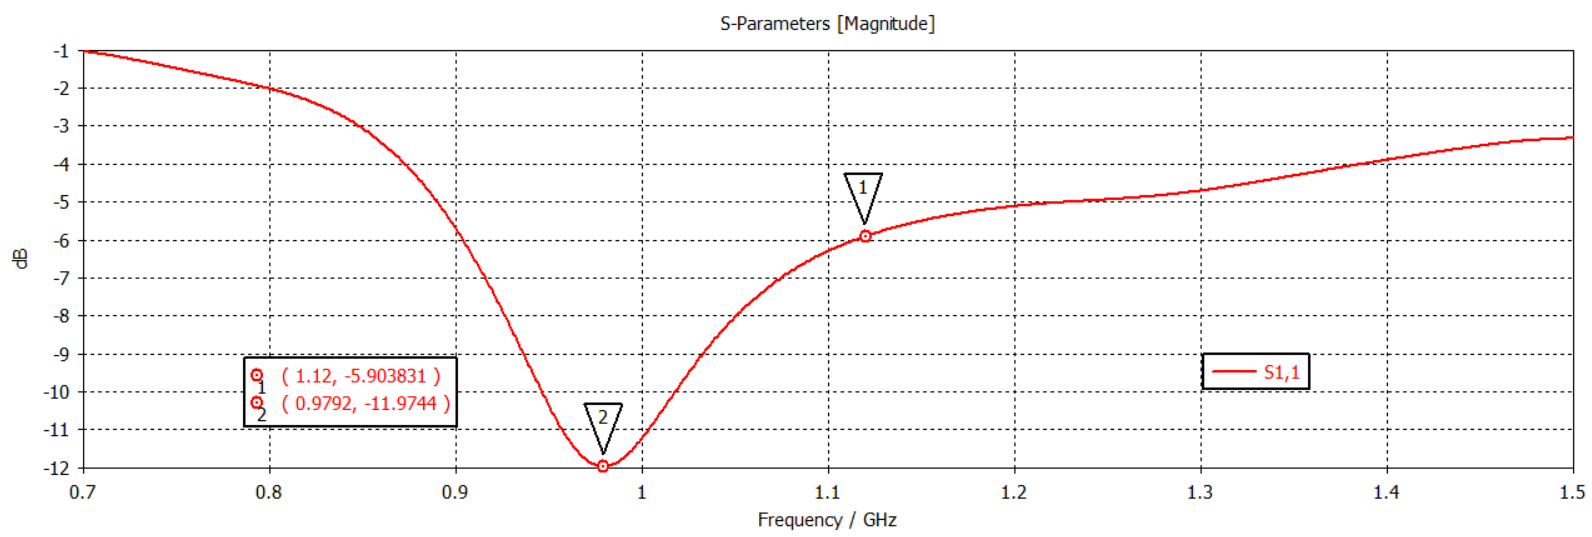
\includegraphics[width=0.82\textwidth]{figures/body_5mm/s11_body_5mm_with_markers.png}
\caption{Return loss for the \(5~\mathrm{mm}\) body-separation case. The matching minimum occurs at \(0.9792~\mathrm{GHz}\), while \(S_{11}\) at \(1.120~\mathrm{GHz}\) is \(-5.903831~\mathrm{dB}\).}
\label{fig:body-5mm-s11}
\end{figure}

\subsubsection{Efficiency and Gain Result}

The far-field result at \(1.120~\mathrm{GHz}\) showed that the \(5~\mathrm{mm}\) body-separation case had lower radiating performance than the \(10~\mathrm{mm}\) case. CST reported the following values:

\[
\eta_{\mathrm{rad}} = -3.837~\mathrm{dB},
\]

\[
\eta_{\mathrm{tot}} = -5.126~\mathrm{dB},
\]

and

\[
G = 0.3534~\mathrm{dBi}.
\]

\begin{table}[htbp]
\centering
\caption{Efficiency and gain result for the \(5~\mathrm{mm}\) body-separation case at \(1.120~\mathrm{GHz}\).}
\label{tab:body-5mm-efficiency-gain}
\begin{tabular}{lc}
\hline
\textbf{Quantity} & \textbf{Value} \\
\hline
Radiation efficiency & \(-3.837~\mathrm{dB}\) \\
Total efficiency & \(-5.126~\mathrm{dB}\) \\
Gain & \(0.3534~\mathrm{dBi}\) \\
\hline
\end{tabular}
\end{table}

The radiation efficiency decreased because the tissue layers were closer to the antenna and absorbed more electromagnetic power. The total efficiency decreased even more because the antenna was also poorly matched at \(1.120~\mathrm{GHz}\). Therefore, the lower total efficiency is the combined result of increased tissue loss and increased impedance mismatch.

The CST far-field parameter summary for the \(5~\mathrm{mm}\) body-separation case is shown in Figure~\ref{fig:body-5mm-farfield-parameters}.

\begin{figure}[htbp]
\centering
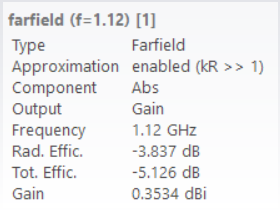
\includegraphics[width=0.42\textwidth]{figures/body_5mm/farfield_parameters_body_5mm.png}
\caption{CST far-field parameter summary for the \(5~\mathrm{mm}\) body-separation case at \(1.120~\mathrm{GHz}\).}
\label{fig:body-5mm-farfield-parameters}
\end{figure}

\subsubsection{Radiation Pattern Observation}

The far-field radiation pattern was evaluated at

\[
1.120~\mathrm{GHz}.
\]

As in the \(10~\mathrm{mm}\) case, the CST far-field monitor reports the far-zone radiation behavior of the complete antenna-body system. The body itself is located in the near-field region of the antenna, but the far-field pattern is obtained after solving the near-field interaction between the dipole and the lossy tissue layers.

For the \(5~\mathrm{mm}\) case, the radiation pattern was more strongly affected by the body than in the \(10~\mathrm{mm}\) case. The maximum gain decreased to

\[
0.3534~\mathrm{dBi},
\]

indicating that less power was radiated effectively into the far field. This reduction is consistent with stronger tissue absorption and stronger perturbation of the current distribution on the dipole.


The three-dimensional gain pattern at \(1.120~\mathrm{GHz}\) is shown in Figure~\ref{fig:body-5mm-3d-pattern}.

\begin{figure}[htbp]
\centering
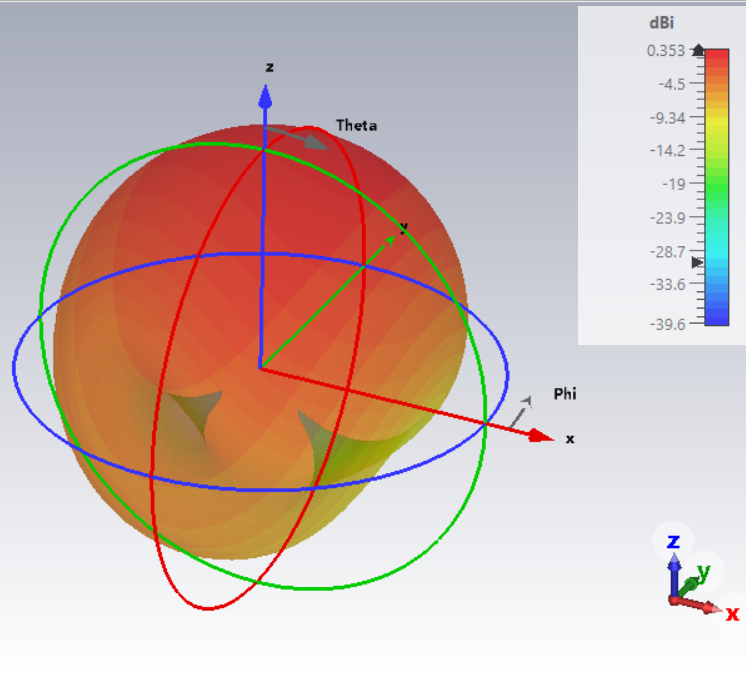
\includegraphics[width=0.82\textwidth]{figures/body_5mm/pattern_3d_gain_body_5mm.png}
\caption{Three-dimensional gain pattern for the \(5~\mathrm{mm}\) body-separation case at \(1.120~\mathrm{GHz}\).}
\label{fig:body-5mm-3d-pattern}
\end{figure}


The E-plane and H-plane radiation-pattern cuts for the \(5~\mathrm{mm}\) body-separation case are shown in Figures~\ref{fig:body-5mm-2d-phi0} and~\ref{fig:body-5mm-2d-phi90}, respectively. Since the dipole is oriented along the \(x\)-axis, the \(\phi=0^\circ\) cut corresponds to the \(x\)-\(z\) principal plane, or E-plane, while the \(\phi=90^\circ\) cut corresponds to the \(y\)-\(z\) principal plane, or H-plane.

\begin{figure}[htbp]
\centering
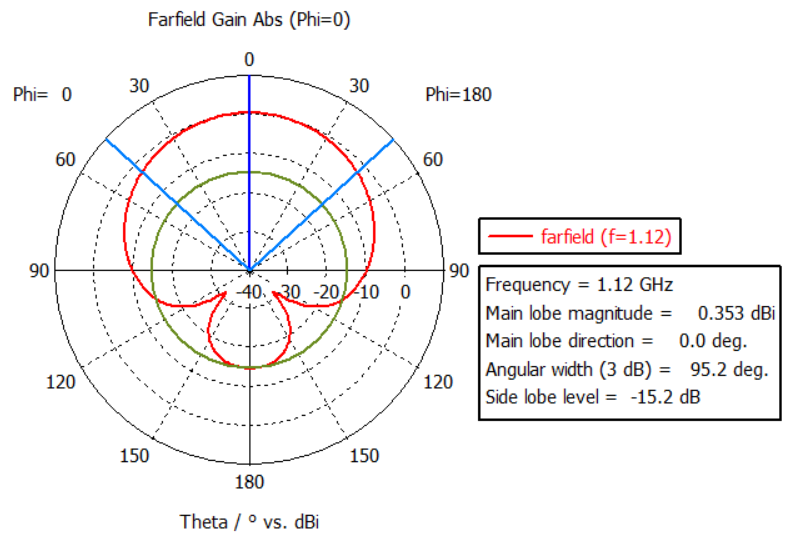
\includegraphics[width=0.82\textwidth]{figures/body_5mm/pattern_2d_body_5mm_phi0.png}
\caption[E-plane radiation-pattern cut for the \(5~\mathrm{mm}\) body-separation case.]
{E-plane radiation-pattern cut for the \(5~\mathrm{mm}\) body-separation case at \(1.120~\mathrm{GHz}\). For the \(x\)-oriented dipole, this cut corresponds to the \(\phi=0^\circ\) principal plane, or the \(x\)-\(z\) plane.}
\label{fig:body-5mm-2d-phi0}
\end{figure}

\begin{figure}[htbp]
\centering
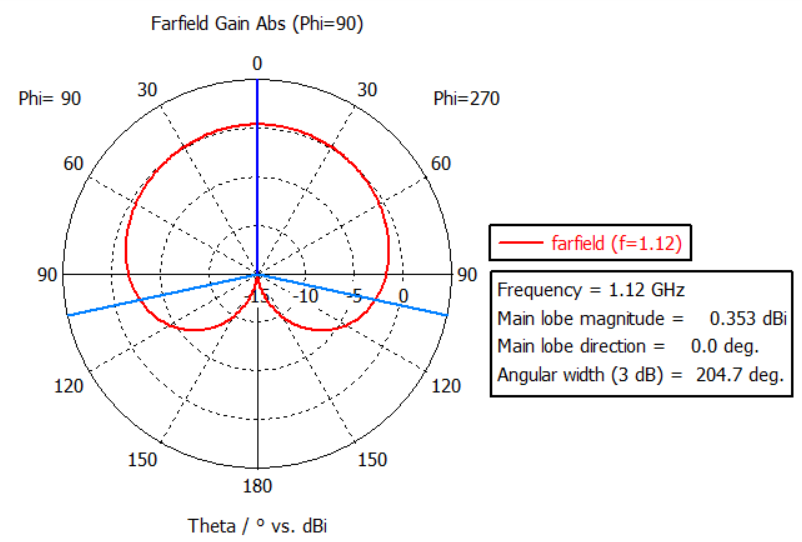
\includegraphics[width=0.82\textwidth]{figures/body_5mm/pattern_2d_body_5mm_phi90.png}
\caption[H-plane radiation-pattern cut for the \(5~\mathrm{mm}\) body-separation case.]
{H-plane radiation-pattern cut for the \(5~\mathrm{mm}\) body-separation case at \(1.120~\mathrm{GHz}\). For the \(x\)-oriented dipole, this cut corresponds to the \(\phi=90^\circ\) principal plane, or the \(y\)-\(z\) plane.}
\label{fig:body-5mm-2d-phi90}
\end{figure}

\subsubsection{Interpretation of the 5 mm Case}

The \(5~\mathrm{mm}\) body-separation case confirms that antenna-body coupling becomes stronger as the antenna is moved closer to the lossy multilayer tissue model. The tuned free-space dipole had its matching minimum near

\[
1.1168~\mathrm{GHz},
\]

whereas the \(5~\mathrm{mm}\) body case produced a matching minimum at

\[
0.9792~\mathrm{GHz}.
\]

This shift corresponds to a significant detuning below the design operating frequency. The physical reason is that the high-permittivity body layers increase the effective electrical loading around the dipole, causing the fixed physical antenna length to behave as if it were electrically longer.

At the target frequency, the return loss degraded to

\[
-5.903831~\mathrm{dB},
\]

which is far above the desired \(-10~\mathrm{dB}\) matching criterion. The gain also dropped to

\[
0.3534~\mathrm{dBi}.
\]

Therefore, the \(5~\mathrm{mm}\) case demonstrates both impedance degradation and radiating-performance degradation. This case was later selected as the main retuning case because it represents a realistic near-body wearable condition and shows a clear downward detuning trend that can be addressed by shortening the dipole.
